\lecture{LECTURE: Interconnection Protocols}{2023-02-07}{09:00}{Amanda}{Zoom}

\section*{Voice Over Internet Protocol}
\textit{Voice over Internet Protocol} (VOIP) was originally created to reduce the need to pay to send to email. However this raises the question, why pay for digitalised voice traffic?

VoIP is commonplace now and will be found in many businesses, the University, for example uses VoIP in place of traditional phones in many locations.

The current motivation behind using VoIP is: to reduce the cost; only need to maintain a single piece of infrastructure (the network, rather than a computer network and telecommunications network); to gain extended capabilities; avoid excess delivery delay; and provide a good QoS. However there are a number of downsides: the quality of the connection may not be great, this depends on the "gateway" between the VoIP phones and legacy telephone networks; and wireless devices may drop connection temporarily when moving between access points. 

\section*{Session Initiation Protocol}
\textit{Session Initiation Protocol} (SIP) is an application layer protocol which provides a single infrastructure for voice, video and instant messaging communications to be transmitted through. SIP started as a way establish a connection, modify a connection and terminate a connection used for calling. SIP is a signalling protocol for real-time sessions.

There are five categories.
\begin{itemize}
    \item User Location - real time local discovery
    \item User availability - is user able to communicate?
    \item User capability - choice of media and coding scheme
    \item Session setup - establishing the session
    \item Session Management - transferring sessions; modifying parameters
\end{itemize}

SIP is similar to HTTP in that SIP and HTTP are both request-response connections.

\section*{The Internet and NAPs}
The internet consists of a hierarchy of \textit{Internet Service Providers} (ISPs) of various sizes
\begin{itemize}
    \item Tier 1 - International ISPs
    \item Tier 2 - National ISPs
    \item Tier 3 - Regional ISPs
    \item Tier 4 - Local ISPs
\end{itemize}

\textit{Network Access Points} (NAPs) are \textit{Internet Exchange Points} (IXPs). They interconnect public peering ISPs to exchange traffic and they exchange routing information using BGP-4. BGP-4 works on service level agreements to allow other companies to use their infrastructure (generally the amount the borrowing company can use is quite high and will have a cost associated if they go over their quota), the SLAs get updated quite frequently. 

Selective Private Peering with direct inter-ISP links. The private aspect of this may be dedicated for some businesses or for ISP use.

NAPs are layer 2 switches, which typically use ATM switching and have support for ISO-provided routers. NAPs are interconnected by high-speed backbones.
\begin{figure}[ht]
    \centering
    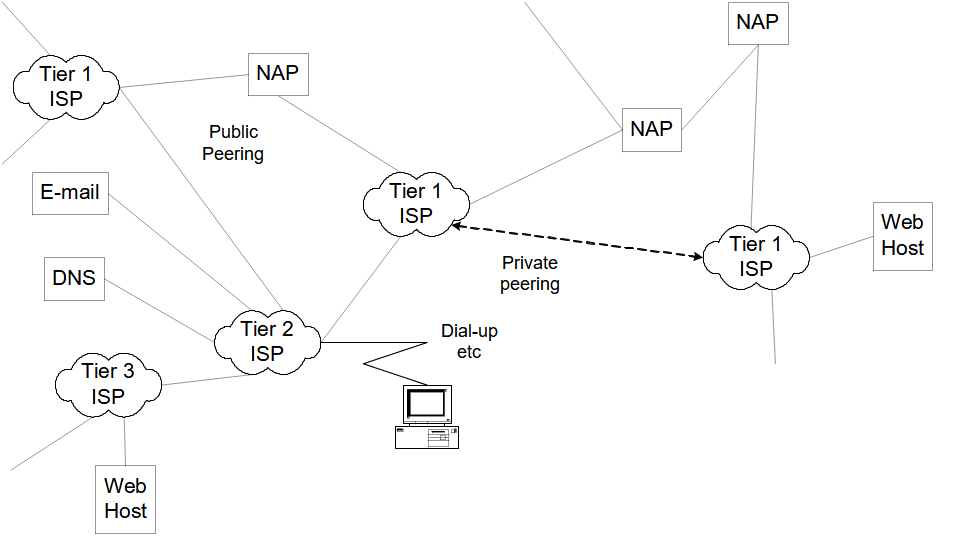
\includegraphics[width=0.9\textwidth]{assets/internet-nap.png}
    \caption*{Diagram of the relationship between NAPs and the internet}
\end{figure}

\section*{Router Capabilities}
There are several different types of routers.
\begin{itemize}
    \item Access Routers - edges of the network (this is the usual type of the domestic router)
    \item Enterprise Routers - Organisation network
    \item Core Routers - Handling heavy data flow
\end{itemize}

Routers may also have layer 2 switching capabilities and they may have hardware or software routing capabilities. Routers can either be table top or chassis based (these can contain multiple plug-in router modules). 
\subsection*{Modern Router Capabilities}
Routers may be embedded into other multi-feature network devices, which also can include
\begin{itemize}
    \item Wireless Access Point (WAP)
    \item A small (for example, 4-port) wired switch
    \item Firewall (usually a standalone hardware device)
\end{itemize}

\section*{Multi Protocol Layer Switching}
\textit{Multi Protocol Layer Switching} MPLS's philosophy is "route at the edges, switch in the core". It provides the best parts of both layer 3 routing control and layer 2 switching. Layer 3 is the "multi-protocol" part of MPLS, since the switch is done at layer 2.

MPLS is intended for use in the core portion of intranets/ the internet. It is useful for carriers, ISPs and enterprise WAN networks. MPLS router int he core is called a \textit{label-switching router} (LSR).

MPLS specifications allow many variations (options). Route the first packet when an MPLS label path doesn't exist to the destination network, as the first packet is processed at each LSR- the layer 2 switched connections is setup between those LSRs. Subsequent packets are handled by switching at layer 2 (eg ATM), swapping the label at each LSR, and label switching is also label swapping. 

\subsection*{A Specific MPLS Approach}
Benefits of MPLS include
\begin{itemize}
    \item Traffic engineering capabilities (explicit path other than that selected by routing)
    \item MPLS-based VPNs with simpler provisioning
    \item Service differentiation (QoS)
    \item Improved performance (switching instead of routing at each hop)
    \item Scalability
\end{itemize}

MPLS brings forward many of the benefits of connection-oriented forwarding to connectionless intranets and their routing protocols. 

\section*{QoS with IP}
QoS usually refers to providing support for time-sensitive delivery, such as voice or compressed video.

Much of the work in this areas is now showing up in products, usually involving prioritisation of traffic based on the type of data being carried.

Effort includes: various forms of IP switching; differentiation services (using the IP TOS byte); multi protocol label switching MPLS